\section{The 35-move construction and its conditional interfaces}
\label{app:route35}

This appendix gives a separate construction from six immediate-completion
cards and 610 further rows.  Besides an ordinary 35-move strategy, it
provides four conditional strategies with small required sets and
specified regions in which Breaker may already have played.  Those
conditional conclusions concern arbitrary prior ownership, so they do
not follow merely from a better bound for the empty board.
We retain both the complete opening and the transfer, opposite-tip, and
bent-shape continuations that explain how this certificate operates.

Throughout this appendix, \(A_i^{35},T_i^{35},h_i^{35}\) denote the required
set, envelope, and height of row \(i\) of the \emph{35-move certificate}.
These indices and the placement codes below are separate from those of
the 21- and 25-move constructions.  The meaning of a card is the
arbitrary-ownership meaning of Section~\ref{sec:calculus}: at any Maker
turn, finite disjoint sets \(M,B\) with
\(A_i^{35}\subseteq M\) and \(B\cap T_i^{35}=\varnothing\) permit a win
within \(h_i^{35}\) further actual Maker claims, unless a target is
already complete.  Additional ownership is allowed everywhere.

\subsection{The letter-and-offset certificate}
\label{r35:decoder}

Write the target points in the fixed order
\[
 s_0=(0,0),\quad s_1=(1,0),\quad s_2=(2,0),\quad
 s_3=(3,0),\quad s_4=(3,1),\quad s_5=(4,1),
 \qquad o=(0,0).
\]
The six initial cards are
\begin{equation}\label{r35:bases}
 T_i^{35}=S-s_i,\qquad
 A_i^{35}=T_i^{35}\setminus\{o\},\qquad h_i^{35}=1
 \quad(0\le i\le5).
\end{equation}
They are valid by immediate completion.  If the missing point is already
Maker-owned, the target has already been obtained.

For \(i=6,\ldots,615\), the literal row consists of \(i\) followed by a
nonempty list of placement terms.  A term \texttt{kLuv} contains an
earlier decimal row index \(k<i\), one letter \(L\), and two individual
decimal digits \(u,v\).  Its placement is
\begin{equation}\label{r35:placement}
 F_{Luv}(x,y)=R_L(x,y)+(u-4,v-4),
\end{equation}
with the eight maps specified by
\begin{center}
\small
\begin{tabular}{c|cccc}
\(L\)&a&b&c&d\\ \hline
\(R_L(x,y)\)&\((x,y)\)&\((y,x)\)&\((x,-y)\)&\((-y,x)\)\\[3pt]
\(L\)&e&f&g&h\\ \hline
\(R_L(x,y)\)&\((-x,y)\)&\((y,-x)\)&\((-x,-y)\)&\((-y,-x)\)
\end{tabular}
\end{center}
Thus \texttt{614b43} means \((x,y)\mapsto(y,x-1)\), including its
translation; it is not one of the decimal orientation codes used in the
other two certificates.

If the terms of row \(i\) are \((k_j,L_ju_jv_j)\), put
\(C_j=F_{L_ju_jv_j}(A_{k_j}^{35})\) and
\(D_j=F_{L_ju_jv_j}(T_{k_j}^{35})\).  Define
\begin{equation}\label{r35:recursion}
 \begin{split}
 T_i^{35}&=\{o\}\cup\bigcup_j D_j,\\
 A_i^{35}&=\left(\bigcup_j C_j\ \cup\ \bigcap_jD_j\right)
             \setminus\{o\},\\
 h_i^{35}&=1+\max_j h_{k_j}^{35}.
 \end{split}
\end{equation}
Lemma~\ref{thm:composition} and induction on \(i\) prove every card
defined in this way.  The inductive argument is valid for every
syntactically correct list of backward references; the particular list
determines the useful required sets and envelopes.

For clarity, the complete finite substitution can be performed as
follows.  Initialize the six triples by \eqref{r35:bases}.  Read each
remaining row in increasing order, reject an empty list or a reference
outside \(0,\ldots,i-1\), decode each affine map by
\eqref{r35:placement}, and apply it to both stored sets.  Take the union
and intersection in \eqref{r35:recursion}, store the resulting triple,
and proceed to the next row.  All coordinates are integers and all sets
are finite.  At the end of each iteration the stored triples are
exactly the triples defined by the displayed equations, which is the
loop invariant justifying the reconstruction.

The complete 610-row literal is printed in Appendix~\ref{app:data35}
and supplied as \nolinkurl{verification/supporting/prior-35/certificate.txt}; it has
one row per line, including the final newline.  The primary and two
independent reconstructions are described in Appendix~\ref{app:checker}.
They use, respectively,
integer matrices and ordinary set operations, quarter turns and
incidence masks, and signed coordinate lookups with cellwise membership
tests.  Thus no search procedure or undisclosed strategy tree is needed
to recover the certificate.

\subsection{The first two compositions: five cells in a row}
\label{r35:elementary}

The first two nonbase rows are
\[
 \texttt{6 0a03},\qquad \texttt{7 4a34 6a54}.
\]
Set
\[
 L_- = \{-4,-3,-2,-1\}\times\{-1\},\qquad
 L_+ = \{-3,-2,-1,0\}\times\{-1\}.
\]
Row 6 has
\[
 T_6^{35}=S+(-4,-1)=L_-\cup\{(-1,0),o\},\qquad
 A_6^{35}=L_-\cup\{(-1,0)\},\qquad h_6^{35}=2.
\]
The height is the recursively assigned upper bound: after claiming its
pivot, Maker has in fact completed this target immediately.

The two placed children in row 7 have
\begin{equation}\label{r35:elementary-children}
\begin{array}{c|c|c}
\text{term}&\text{required set}&\text{envelope}\\ \hline
\texttt{4a34}&L_-\cup\{o\}&L_-\cup\{(-1,0),o\}\\
\texttt{6a54}&L_+\cup\{o\}&L_+\cup\{o,(1,0)\}.
\end{array}
\end{equation}
Their common envelope is
\((\{-3,-2,-1\}\times\{-1\})\cup\{o\}\), already contained in the
union of their required sets.  Consequently
\[
 A_7^{35}=\{-4,-3,-2,-1,0\}\times\{-1\},\qquad
 T_7^{35}=A_7^{35}\cup\{(-1,0),o,(1,0)\},\qquad h_7^{35}=3.
\]
After Maker owns the five lower cells and the pivot \(o\), either
\((-1,0)\) or \((1,0)\) completes one of the two displayed copies.
Both lie in the parent envelope, so neither is occupied by an earlier
Breaker stone.  If neither target is already complete, Breaker can
claim at most one of these two cells.  This is the elementary double
threat that the longer compositions reuse.  Its direct two-claim bound
is sharper than the stored height 3; the certificate deliberately uses
the uniform recursion \eqref{r35:recursion}.

\subsection{Four conditional outputs}
\label{r35:outputs}

The following finite identities supply the opening.  A set in the last
column is wholly disjoint from the envelope; it is not asserted to be
the entire complement of that envelope.

\begin{proposition}\label{r35:conditional}
The 35-move certificate has 616 cards, including its six base cards,
and 1,837 placement terms.  Every card satisfies
\(A_i^{35}\subsetneq T_i^{35}\),
\(o\in T_i^{35}\setminus A_i^{35}\), and \(h_i^{35}\le34\).
Four of its conditional interfaces are
\begin{equation}\label{r35:conditional-table}
\begin{array}{c|c|r|r|l}
 i&A_i^{35}&|T_i^{35}|&h_i^{35}&\text{region disjoint from }T_i^{35}\\ \hline
 557&\{(-1,0)\}&118&19&\{(x,y):x\le-3,\ y\le-2\}\\
 595&\{(-1,0)\}&222&27&\{(x,y):x=-2,\ y\le-2\}\\
 603&\{(-1,0)\}&275&27&\{(x,y):x\le-3,\ y=0\}\\
 615&\{(1,0)\}&686&34&\{(1,-1)\}.
\end{array}
\end{equation}
Each row applies at any Maker turn with its required point owned and
its entire envelope free of Breaker, regardless of all other ownership.
For row 615 there is also a Breaker-turn conclusion: if Maker owns
\(\{o,(1,0)\}\) and Breaker avoids \(T_{615}^{35}\), then after any
legal next reply Maker wins within 33 further claims, unless already
victorious.
\end{proposition}

\begin{proof}
The finite identities follow by the substitutions
\eqref{r35:bases}--\eqref{r35:recursion}.  The delivered reconstructions
check every row index, every placement and backward reference, the full
sets and heights, and the four outputs in
\eqref{r35:conditional-table}.  An omitted infinite region is checked
by testing its defining predicate at \emph{every} point of the finite
envelope.  For example, the first check verifies
\(x>-3\) or \(y>-2\) for every \((x,y)\in T_{557}^{35}\); this proves
disjointness from the whole infinite region, without sampling it.

For each composed card the reconstruction also verifies
\(C_j\subseteq A_i^{35}\cup\{o\}\) and \(D_j\subseteq T_i^{35}\).
It checks each possibly legal local reply in
\(T_i^{35}\setminus(A_i^{35}\cup\{o\})\), and one extra class
representing all cells outside \(T_i^{35}\).  There are 26,703 such classes in total over
the 610 composed rows.  In each class some child envelope is missed.
The exterior class is exact because every child envelope is contained
in the parent envelope.  Extra Maker ownership can only remove legal
reply cells, and earlier Breaker ownership is excluded by the envelope
hypothesis.  These checks establish the stated finite identities; the
game-theoretic conclusion is the induction using
Lemma~\ref{thm:composition}, not an inference from the number of tests.
Its Breaker-turn assertion gives the final claim, since
\(h_{615}^{35}-1=33\).
\end{proof}

\subsection{The complete ordinary opening}
\label{r35:opening}

\begin{theorem}\label{r35:theorem}
There is one ordinary Maker policy on the initially empty infinite
square board that completes an allowed copy of \(S\) within 35 actual
Maker claims against every legal Breaker play.  Equivalently, after
extending a won position by fresh moves if necessary, its 35th Maker
set contains a target whenever the first 34 Breaker replies are legal.
No 35th Breaker reply is required.
\end{theorem}

\begin{proof}
Maker first claims the actual origin.  Write \(q_*\ne o\) for Breaker's
first cell, and let \(0\le a\le b\) be the sorted absolute values of its
two coordinates.  Since the cell differs from the origin, \(b\ge1\).
We first handle all unbounded distant replies, and then the eight
adjacent or diagonal replies.

Suppose \(b\ge2\).  In local coordinates put \(p=(-1,0)\), and choose
\begin{equation}\label{r35:distant-choice}
 (i,d)=
 \begin{cases}
 (557,(-a,-b)),&a\ge2,\\
 (595,(-1,-b)),&a=1,\\
 (603,(-b,0)),&a=0.
 \end{cases}
\end{equation}
In each case \(d\) and \(q_*\) have the same sorted absolute
coordinates, so there is a signed permutation \(R\in\mathcal G\) with
\(Rd=q_*\).  Use the affine map
\begin{equation}\label{r35:opening-map}
 F(z)=R(z-p).
\end{equation}
It sends the required cell \(p\) to Maker's first cell, and the local
Breaker cell \(p+d\) to \(q_*\).  In the three respective cases,
\[
 p+d=(-a-1,-b),\qquad (-2,-b),\qquad (-b-1,0).
\]
The first has \(x\le-3,y\le-2\), the second has \(x=-2,y\le-2\), and
the third has \(x\le-3,y=0\).  Thus it lies in the corresponding
omitted region in \eqref{r35:conditional-table}.  At Maker's second
turn, \(F(A_i^{35})\) is owned and \(F(T_i^{35})\) contains no Breaker
cell.  The placed conditional card applies, giving totals at most
\(1+19=20\), \(1+27=28\), and \(1+27=28\), respectively.  The
argument used no upper bound on \(a\) or \(b\).

It remains to treat \(b=1\).  Put
\[
 q=(1,-1),\qquad P=\{o,(1,0)\},\qquad
 p=\begin{cases}(1,0),&a=0,\\o,&a=1.\end{cases}
\]
For the coordinate-adjacent reply, \(q-p=(0,-1)\); for the diagonal
reply, \(q-p=(1,-1)\).  In either case choose \(R\in\mathcal G\) with
\(R(q-p)=q_*\), and again use \eqref{r35:opening-map}.  Then
\(F(p)=o\) and \(F(q)=q_*\).  Maker's second move claims the other
cell of \(F(P)\).  It is fresh: the two cells of \(P\) differ, and
\(q\notin P\).  Immediately after this move,
\[
 M=F(P)=F(A_{615}^{35}\cup\{o\}),\qquad
 B=\{F(q)\},\qquad B\cap F(T_{615}^{35})=\varnothing.
\]
The two Maker cells have been obtained with the actual first Breaker
reply between them.  In the adjacent case the local pivot \(o\) was
played second; in the diagonal case it was played first.  This order
does not matter to the state-based Breaker-turn assertion of
Proposition~\ref{r35:conditional}.

It is now Breaker's second turn.  Every legal reply misses at least
one child envelope of the placed row 615, with that child's required
set already owned.  The child wins within at most 33 further Maker
claims.  Thus the total in the near case is
\[
 2+33=35.
\]
Figure~\ref{r35:near-figure} records both possible orders of the domino.

\begin{figure}[tb]
\centering
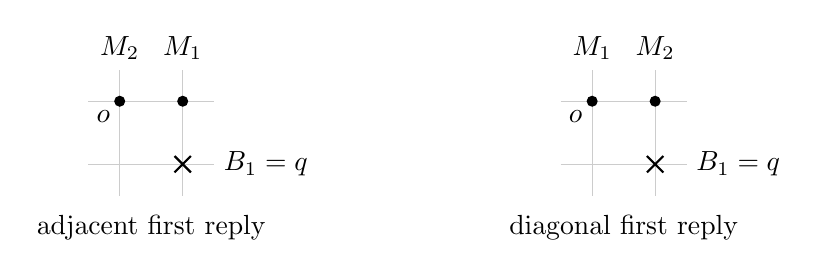
\begin{tikzpicture}[x=8mm,y=8mm]
\begin{scope}
\draw[gray!40,step=1] (-.5,-1.5) grid (1.5,.5);
\fill (0,0) circle (2pt); \fill (1,0) circle (2pt);
\node[above] at (0,.5) {$M_2$}; \node[above] at (1,.5) {$M_1$};
\node[below left] at (0,0) {$o$};
\draw[thick] (.87,-1.13)--(1.13,-.87) (.87,-.87)--(1.13,-1.13);
\node[right] at (1.5,-1) {$B_1=q$};
\node at (.5,-2) {adjacent first reply};
\end{scope}
\begin{scope}[xshift=6cm]
\draw[gray!40,step=1] (-.5,-1.5) grid (1.5,.5);
\fill (0,0) circle (2pt); \fill (1,0) circle (2pt);
\node[above] at (0,.5) {$M_1$}; \node[above] at (1,.5) {$M_2$};
\node[below left] at (0,0) {$o$};
\draw[thick] (.87,-1.13)--(1.13,-.87) (.87,-.87)--(1.13,-1.13);
\node[right] at (1.5,-1) {$B_1=q$};
\node at (.5,-2) {diagonal first reply};
\end{scope}
\end{tikzpicture}
\caption{Local coordinates immediately after Maker's second claim and
before Breaker's second reply.  Dots are Maker's domino \(P\), the
cross is the existing Breaker cell \(q\), and subscripts show the order
of the actual moves.  Row 615 controls the next reply in both cases.}
\label{r35:near-figure}
\end{figure}

Fix the choices before play: order the eight signed permutations and
the terms in every row, and fix an enumeration of \(\mathbb Z^2\).
Use the first admissible opening matrix and the first child envelope
missed by the latest reply.  Compose each child map with the current
affine frame.  If its pivot is already Maker-owned and no target is
complete, claim the first genuinely free cell in the enumeration;
that replacement and the following legal reply are charged in the
height recursion.  Every child has smaller index, so the recursion
terminates within the stated height.  On histories inconsistent with
earlier prescriptions, use the first free cell.  This gives one total
fresh policy, with the same early-stopping and extension conventions as
Section~\ref{sec:strategy}.  An extended 35-claim play contains only
34 intervening Breaker replies, proving the precise endpoint.
\end{proof}

\subsection{Transferring a four-cell attack to a new pair}
\label{r35:transfer}

We now examine the longer tactics inside the certificate.  They explain
how a small required set can support a continuation even after several
forced parries.  The conditions always concern the entire envelope;
the visible stones alone do not license a card.

Put \(V=\{-1\}\times\{-4,-3,-2,-1\}\).  The relevant literal rows and
reconstructed outputs are
\[
 \texttt{588 3b33 586a45},\qquad
 \texttt{589 4b43 588a45},
\]
\begin{equation}\label{r35:transfer-data}
\begin{array}{c|c|r|r}
i&A_i^{35}&|T_i^{35}|&h_i^{35}\\ \hline
586&\{(0,-2),(0,-1)\}&198&26\\
588&(V\setminus\{(-1,-1)\})\cup\{(0,-1)\}&202&27\\
589&V&204&28.
\end{array}
\end{equation}
Their envelopes satisfy the more informative identities
\begin{equation}\label{r35:transfer-envelopes}
\begin{split}
T_{588}^{35}&=(T_{586}^{35}+(0,1))\cup V,\\
T_{589}^{35}&=(T_{586}^{35}+(0,2))
 \cup (\{-1\}\times\{-4,-3,-2,-1,0\})\cup\{(0,-1)\}.
\end{split}
\end{equation}
In particular, each smaller continuation envelope is contained in the
envelope under which the tactic starts.

For an explicit description of these envelopes, Table~\ref{r35:fibers}
gives every vertical fiber of \(T_{586}^{35}\).  In this table
\([a,b]_{\mathbb Z}\) means every integer from \(a\) to \(b\), and
unlisted fibers are empty.  Together with
\eqref{r35:transfer-envelopes}, it specifies all three complete
envelopes, including cells far from the initial column.
\begin{table}[tb]
\centering\small
\begin{tabular}{c|l@{\qquad}c|l@{\qquad}c|l}
\(x\)&\(\{y:(x,y)\in T_{586}^{35}\}\)&
\(x\)&\(\{y:(x,y)\in T_{586}^{35}\}\)&
\(x\)&\(\{y:(x,y)\in T_{586}^{35}\}\)\\ \hline
\(-7\)&\([3,4]_{\mathbb Z}\cup\{6\}\)&0&\([-2,9]_{\mathbb Z}\)&7&\([-5,5]_{\mathbb Z}\)\\
\(-6\)&\(\{1\}\cup[3,6]_{\mathbb Z}\)&1&\([-6,9]_{\mathbb Z}\)&8&\([-2,4]_{\mathbb Z}\)\\
\(-5\)&\([-1,9]_{\mathbb Z}\)&2&\([-7,9]_{\mathbb Z}\)&9&\([-2,4]_{\mathbb Z}\)\\
\(-4\)&\([-1,8]_{\mathbb Z}\)&3&\([-6,9]_{\mathbb Z}\)&10&\([-2,0]_{\mathbb Z}\)\\
\(-3\)&\([-1,11]_{\mathbb Z}\)&4&\([-7,7]_{\mathbb Z}\)&11&\(\{-2,0\}\)\\
\(-2\)&\([-2,10]_{\mathbb Z}\)&5&\([-5,6]_{\mathbb Z}\)&&\\
\(-1\)&\([-1,11]_{\mathbb Z}\)&6&\([-5,6]_{\mathbb Z}\)&&
\end{tabular}
\caption{The complete 198-cell envelope of row 586.  The translated
envelopes governing the two forced parries and the transferred pair
follow from \eqref{r35:transfer-envelopes}.}
\label{r35:fibers}
\end{table}

Suppose \(V\subseteq M\) and \(B\cap T_{589}^{35}=\varnothing\) at a
Maker turn.  Claim \(o\) (or make the charged fresh replacement if it
is already owned).  The set
\[
 Q_1=V\cup\{o,(0,-1)\}
\]
is the target in the placed base card \texttt{4b43}.  Its only possibly
missing Maker cell is \((0,-1)\).  If this point is already owned,
Maker has won.  Otherwise it is free, because it lies in the parent
envelope.  A Breaker reply other than \((0,-1)\) leaves that immediate
completion available, so any defense avoiding this win must claim
\((0,-1)\).

The other child \texttt{588a45} uses the map \(z\mapsto z+(0,1)\).
Its required set is
\[
 (\{-1\}\times\{-3,-2,-1\})\cup\{o\},
\]
which is contained in the Maker set.  Its envelope
\(T_{588}^{35}+(0,1)\) is a subset of \(T_{589}^{35}\) and omits
\((0,-1)\).  All Breaker cells, including that first parry, therefore
avoid it.  Claim its pivot \((0,1)\), with the same charged-replacement
convention if necessary.  Now
\[
 Q_2=\{(-1,-3),(-1,-2),(-1,-1),(-1,0),o,(0,1)\}
\]
is complete except possibly at \((-1,0)\).  It is another allowed
target: \(Q_1=R_b(S)+(-1,-4)\) and
\(Q_2=R_b(S)+(-1,-3)\).  Thus, unless Maker has already won or can
complete \(Q_2\) on the next move, Breaker must parry at \((-1,0)\).

After these two parries, the continuation \texttt{586a45} of the
translated row 588 is row 586 translated by \((0,2)\).  Its required
set is exactly \(\{o,(0,1)\}\), now owned.  Its envelope
\[
 D=T_{586}^{35}+(0,2)
\]
lies in the original envelope and contains neither parry:
\((0,-1)\notin D\) and \((-1,0)\notin D\).  These omissions follow
directly from the fibers \(x=0\) and \(x=-1\) in
Table~\ref{r35:fibers}.  The envelope of the preceding row-588
continuation likewise omits the first parry by
\eqref{r35:transfer-envelopes}.  Row 586 therefore applies at the next
Maker turn, with pivot \((0,2)\) and bound 26.  The two earlier claims
and their forced replies have transferred the attack from the original
column to a new vertical pair, at total cost at most
\(1+1+26=28\) Maker claims.

This argument preserves every earlier Breaker restriction: all earlier
Breaker cells lie outside the original envelope and hence outside every
continuation envelope.  Extra Maker cells may complete a target early
or occupy one of the prescribed pivots; in the latter case a genuinely
fresh replacement uses the same charged turn.  No assumption that the
displayed stones are the only owned stones is needed.

\subsection{Opposite-tip continuations from four in a row}
\label{r35:opposite}

Row 612 consists exactly of
\[
 \texttt{612 589b55 589h03}.
\]
Writing
\[
 W=\{-3,-2,-1,0\}\times\{0\},\qquad
 G_+(x,y)=(y+1,x+1),\quad
 G_-(x,y)=(-y-4,-x-1),
\]
the two placed requirements are both \(W\), and their envelopes obey
\begin{equation}\label{r35:opposite-intersection}
 G_+(T_{589}^{35})\cap G_-(T_{589}^{35})=W.
\end{equation}
Consequently
\[
 A_{612}^{35}=W\setminus\{o\},\qquad
 T_{612}^{35}=G_+(T_{589}^{35})\cup G_-(T_{589}^{35}),\qquad
 |T_{612}^{35}|=404,\quad h_{612}^{35}=29.
\]
After Maker adds the pivot, \(W\) is owned.  A legal Breaker reply
therefore cannot belong to both child envelopes; choose a child whose
envelope it misses.  All earlier Breaker cells avoid both envelopes by
the parent hypothesis, and the full required column of the selected
copy of row 589 is already owned.  Its next pivot is either \((1,1)\)
or \((-4,-1)\), so the two attacks leave from opposite ends of the
four-cell row.  The transferred pair in the selected frame is
\(G_+(\{o,(0,1)\})\) or \(G_-(\{o,(0,1)\})\), respectively.
Identity~\eqref{r35:opposite-intersection} is what ensures a safe
continuation against every reply, including replies far from the
displayed four stones.

The overlap identity can also be read directly from
Table~\ref{r35:fibers} and \eqref{r35:transfer-envelopes}.  The vertical
supports of the two placed envelopes are \([-6,12]_{\mathbb Z}\) and
\([-12,6]_{\mathbb Z}\), respectively.  On their common possible levels
\(-6\le y\le6\), the fibers have separated extrema for every
\(y\ne0\): the rightmost point of the \(G_-\) fiber is strictly left
of the leftmost point of the \(G_+\) fiber.  At \(y=0\), the
\(G_+\) fiber is \([-3,14]_{\mathbb Z}\) and the \(G_-\) fiber is
\([-17,0]_{\mathbb Z}\).  Their overlap is \([-3,0]_{\mathbb Z}\).
This gives exactly \(W\), and also explains
the envelope count \(204+204-4=404\).

\subsection{The exceptional bent-shape continuation}
\label{r35:exception}

The near opening reaches the local Breaker-turn position with
\(P=\{o,(1,0)\}\) owned and \(q=(1,-1)\) occupied by Breaker.
Here the twelve child terms of row 615 are
\begin{center}
\begin{tabular}{llll}
\texttt{602h64}&\texttt{614b43}&\texttt{533f64}&\texttt{590h64}\\
\texttt{611g34}&\texttt{587d34}&\texttt{601f64}&\texttt{406b64}\\
\texttt{591d34}&\texttt{586d34}&\texttt{584f64}&\texttt{406d34}.
\end{tabular}
\end{center}
For each term let \(C_j,D_j\) be its placed requirement and envelope.
Every \(C_j\) equals \(P\), all \(D_j\) avoid \(q\), and their full
intersection is \(P\).  On deleting the second term, the intersection
becomes
\begin{equation}\label{r35:exception-intersection}
 \bigcap_{j:\,\text{term}_j\ne\texttt{614b43}}D_j
       =P\cup\{(-1,0)\}.
\end{equation}
The next pivots in these eleven children are end extensions
\((-1,0)\) or \((2,0)\).  Since Breaker cannot claim a point of \(P\),
one of them survives every next reply except \((-1,0)\).  Against that
exceptional reply, the only surviving child is \texttt{614b43}.
Its map and pivot are
\[
 K(x,y)=(y,x-1),\qquad K(o)=(0,-1).
\]
The pivot is fresh in the near-opening position: it differs from both
Maker points and both Breaker points \(q,(-1,0)\).

More explicitly,
\[
 A_{614}^{35}=\{(1,0),(1,1)\},\qquad
 K(A_{614}^{35})=P,\qquad |T_{614}^{35}|=678,\qquad h_{614}^{35}=33.
\]
The complete envelope \(K(T_{614}^{35})\) lies in \(T_{615}^{35}\)
and avoids both existing Breaker cells.  An exact expression for the
difference is
\begin{equation}\label{r35:exception-difference}
\begin{split}
 T_{615}^{35}\setminus K(T_{614}^{35})
  =\{&(-15,0),(-15,2),(-14,0),(-14,1),\\
     &(-14,2),(-13,-4),(-13,4),(-1,0)\}.
\end{split}
\end{equation}
Thus the exceptional reply is excluded by the \emph{full} continuation
envelope, not merely by the three-cell configuration that Maker will
obtain.

After Maker claims \((0,-1)\), write
\(Q=P\cup\{(0,-1)\}\).  The seven children of row 614, composed with
\(K\), are listed in Table~\ref{r35:exception-children}.  In the table
the term in the second column is expressed directly in the local
coordinates of the near opening.  For example,
\(K\circ F_{b75}(x,y)=(x+1,y+2)=F_{a56}(x,y)\).

\begin{table}[tb]
\centering\small
\begin{tabular}{c|c|c|r|r}
\text{row-614 term}&\text{term after }K&\text{next pivot}
 &\text{envelope size}&\text{height}\\ \hline
\texttt{608b75}&\texttt{608a56}&\((1,2)\)&354&32\\
\texttt{543d56}&\texttt{543c64}&\((2,0)\)&55&11\\
\texttt{370g34}&\texttt{370h42}&\((0,-2)\)&35&11\\
\texttt{392h34}&\texttt{392g42}&\((0,-2)\)&41&11\\
\texttt{610d56}&\texttt{610c64}&\((2,0)\)&343&32\\
\texttt{600a64}&\texttt{600b45}&\((0,1)\)&259&29\\
\texttt{613a64}&\texttt{613b45}&\((0,1)\)&563&30.
\end{tabular}
\caption{All seven continuations after the exceptional pivot.  Every
placed child requires exactly \(Q=\{o,(1,0),(0,-1)\}\).  Several
children have the same pivot but different complete envelopes.}
\label{r35:exception-children}
\end{table}

Let \(C'_j,D'_j\) be the placed sets of these seven terms.  Their
reconstructed identities are
\begin{equation}\label{r35:exception-coverage}
 C'_j=Q\quad\text{for every }j,\qquad
 \bigcap_{j=1}^7D'_j=Q,\qquad
 D'_j\subseteq K(T_{614}^{35})\quad\text{for every }j.
\end{equation}
The last inclusion excludes both old Breaker stones from every child
envelope.  Any legal third Breaker reply lies outside \(Q\), so the
intersection identity supplies a child envelope it misses.  Its
required set is already owned, and its height is at most 32.  The
selected pivot belongs to that envelope and is outside \(Q\); hence
neither an old Breaker cell nor the new reply occupies it.  It is
therefore fresh in this exact opening position.  The full conditional
version permits extra Maker ownership and uses a charged replacement
if that pivot was owned previously.

The four distinct possible pivots are
\((0,1),(0,-2),(2,0),(1,2)\), as shown in
Figure~\ref{r35:bent-figure}.  They are alternatives selected
\emph{after} the next Breaker reply, rather than a prescribed sequence
of four Maker moves.  The seven distinct envelopes in
\eqref{r35:exception-coverage} determine which alternative is valid;
the visible bent shape by itself does not justify any arbitrary
choice.  The bound after the exceptional second reply is
\(1+32=33\) further Maker claims, including the bent-shape pivot,
which agrees with the \(2+33=35\) opening calculation.

\begin{figure}[tb]
\centering
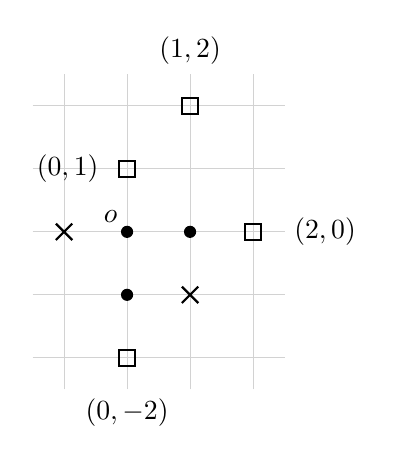
\begin{tikzpicture}[x=8mm,y=8mm]
\draw[gray!35,step=1] (-1.5,-2.5) grid (2.5,2.5);
\foreach \x/\y in {0/0,1/0,0/-1}{\fill (\x,\y) circle (2.2pt);}
\foreach \x/\y in {1/-1,-1/0}{
 \draw[thick] (\x-.13,\y-.13)--(\x+.13,\y+.13)
              (\x-.13,\y+.13)--(\x+.13,\y-.13);}
\foreach \x/\y in {0/1,0/-2,2/0,1/2}{
 \draw[thick] (\x-.13,\y-.13) rectangle (\x+.13,\y+.13);}
\node[above left] at (0,0) {$o$};
\node[right] at (2.5,0) {$(2,0)$};
\node[left] at (-.3,1) {$(0,1)$};
\node[above] at (1,2.5) {$(1,2)$};
\node[below] at (0,-2.5) {$(0,-2)$};
\end{tikzpicture}
\caption{After the exceptional reply \((-1,0)\) and Maker's claim
\((0,-1)\), the filled dots form \(Q\) and the crosses are the two
Breaker cells.  Hollow squares mark possible pivots after Breaker's
next reply.  The diagram displays their geometry; their availability
is determined by the seven envelopes specified by the terms in
Table~\ref{r35:exception-children}.}
\label{r35:bent-figure}
\end{figure}
